% ==========================================
% LatexRefinement Step Output: step4-03-24-25-tuesday-all-offset-final.tex
% Model: gemini-3-flash-preview
% Temperature: 0.36
% TopP: 0.95
% TopK: 40
% MaxOutputTokens: 65535
% ThinkingBudget: 32765
% ThinkingLevel: HIGH
% Prompt Tokens: 35'888
% Candidates Tokens: 18'392 (inkl. Thinking Tokens)
% Cached Tokens: 0
% Processed on: 2026-07-12 09:18:11
% ==========================================

% Primary Language: German

\lecturechapter[6]{Dienstag}{24. Mär}{24. März 2026}{Konstruktion der reellen Zahlen}

\begin{nice-box}[Kontext \& Syllabus]
In dieser Vorlesung wird die formale Konstruktion der reellen Zahlen $\mathbb{R}$ aus den rationalen Zahlen $\mathbb{Q}$ mittels \newterm{Dedekindscher Schnitte} eingeführt. Zuvor erfolgt ein Rückblick auf die Zermelo-Fraenkel-Axiome (ZFC), insbesondere das Fundierungsaxiom, und eine Einordnung des Vollständigkeitsaxioms in den mengentheoretischen Kontext.

\textbf{Syllabus:}
\begin{enumerate}[label=\textbf{(\arabic*)}]
    \item \textbf{Wiederholung:} ZFC-Axiome und das Fundierungsaxiom.
    \item \textbf{Einführung:} Historischer Kontext und Richard Dedekind.
    \item \textbf{Axiomatik:} Das Axiomensystem der reellen Zahlen $\mathbb{R}$.
    \item \textbf{Konstruktion:} Definition und Eigenschaften Dedekindscher Schnitte.
    \item \textbf{Arithmetik:} Addition, Multiplikation und Ordnung auf $\mathbb{R}$.
    \item \textbf{Vollständigkeit:} Beweis des Vollständigkeitsaxioms für Schnitte.
    \item \textbf{Ausblick:} Alternative Konstruktionen (Cauchy-Folgen, quasi-lineare Funktionen).
\end{enumerate}
\end{nice-box}

\section{Einführung und Wiederholung}

\subsection{Das Vollständigkeitsaxiom als Clicker-Frage}
\begin{spoken-clean}[00:00:00 - 00:01:45]
Hallo und herzlich willkommen! Ich habe hier eine kleine Clicker-Einstiegsfrage, die Sie auf der Edu-App beantworten können --- eine gute Gelegenheit, um sich kurz zu konzentrieren. Und wenn Sie das gemacht haben, sagen Sie noch kurz Ihrer Nachbarin oder Ihrem Nachbarn Hallo, und dann bitte wählen.

Gut, wählen Sie noch schnell. $60$ Antworten sollten wir schon noch hinkriegen. Okay, tipptopp. Sehr gut, fast $100\,\%$ richtig --- oder $100\,\%$ richtig, ja, keine falschen Aussagen zumindest.
\end{spoken-clean}

\begin{meta-note}[Projizierter Inhalt: Clicker-Frage]
Der Dozent projiziert eine Clicker-Frage mit einer logischen Formel und vier Antwortmöglichkeiten. Die Formel beschreibt die Existenz des Supremums für nichtleere, nach oben beschränkte Teilmengen der reellen Zahlen.
\end{meta-note}

\begin{math-stroke}[Das Vollständigkeitsaxiom als Clicker-Frage]
\qt{Was sagt die folgende Aussage aus?}
\begin{equation}
\label{eq:clicker-formel}
\begin{aligned}
    &\forall X \subseteq \mathbb{R} \colon \Bigl[ \bigl( X \neq \emptyset \land \exists r \in \mathbb{R} \; \forall x \in X \colon x \le r \bigr) \\
    &\implies \exists s \in \mathbb{R} \colon \bigl( \forall x \in X \colon x \le s \land \forall t \in \mathbb{R} \, (\forall x \in X \colon x \le t \implies s \le t) \bigr) \Bigr]
\end{aligned}
\end{equation}

\textbf{Antwortmöglichkeiten:}
\begin{itemize}
    \item \textbf{1.} Falls $X$ nichtleer und nach oben beschränkt ist, hat $X$ ein Infimum.
    \item \textbf{2.} \textbf{Falls $X$ nichtleer und nach oben beschränkt ist, hat $X$ ein Supremum.} (Korrekte Antwort)
    \item \textbf{3.} Falls $X$ nichtleer und nach unten beschränkt ist, hat $X$ ein Infimum.
    \item \textbf{4.} Falls $X$ nichtleer und nach unten beschränkt ist, hat $X$ ein Supremum.
\end{itemize}

\begin{explanation-of-steps}[Struktur der Formel]
Die Formel \eqref{eq:clicker-formel} lässt sich wie folgt dekonstruieren:
\begin{itemize}
    \item \textbf{Voraussetzung:} $X$ ist eine nichtleere Teilmenge von $\mathbb{R}$ ($X \neq \emptyset$), die eine obere Schranke $r$ besitzt ($\exists r \in \mathbb{R} \; \forall x \in X \colon x \le r$).
    \item \textbf{Konsequenz:} Es existiert eine reelle Zahl $s$, die:
    \begin{enumerate}[label=\textbf{(\arabic*)}]
        \item \textbf{Obere Schranke:} eine obere Schranke von $X$ ist ($\forall x \in X \colon x \le s$), und
        \item \textbf{Kleinste obere Schranke:} die kleinste aller oberen Schranken $t$ ist ($\forall t \in \mathbb{R} \colon (\forall x \in X \colon x \le t) \implies s \le t$).
    \end{enumerate}
\end{itemize}
Diese Zahl $s$ wird als \newterm{Supremum} bezeichnet. Die gesamte Aussage ist das \newterm{Vollständigkeitsaxiom} der reellen Zahlen.
\end{explanation-of-steps}
\end{math-stroke}

\begin{spoken-clean}[00:01:45 - 00:03:45]
Genau, das ist es, was diese Aussage aussagt. Man muss einfach mal genau schauen: Für alle Teilmengen $X$ von $\mathbb{R}$, sodass $X$ nicht leer ist --- also für alle $X$, sodass $X \subseteq \mathbb{R}$ und $X \neq \emptyset$ --- und es existiert ein $r$, sodass für alle $x \in X$ gilt $x \le r$, folgt, dass ein $s$ existiert, sodass für alle $x \in X$ gilt $x \le s$, und für alle $t$, sodass für alle $x \in X$ gilt $x \le t$, dann ist $s \le t$. Dieses $s$ ist hier also das Supremum. Wir wollen also: Wenn $X$ beschränkt ist, dann soll ein solches Supremum existieren, das heißt eine obere Schranke, die die \qt{kleinste} obere Schranke ist.

Dies nur als eine kleine Aufwärmübung. Wie Sie sehen, wird heute das Hauptthema der Vorlesung die Konstruktion der reellen Zahlen sein. Sie haben ja schon viel mit den reellen Zahlen gearbeitet und arbeiten wahrscheinlich auch aktuell viel damit, aber Sie haben noch nie eine volle Konstruktion davon gesehen. Das werden wir hier noch nachholen, wenn auch nicht in allen Details, weil das doch recht mühsam ist.

Zuerst möchte ich aber noch ganz kurz die Sache mit den Zermelo-Fraenkel-Axiomen anschauen. Warten Sie mal schnell... damit ich das Richtige zeige... hier.
\end{spoken-clean}

\begin{meta-note}[Projizierter Inhalt: Die Zermelo-Fraenkel Axiome]
Der Dozent zeigt eine Folie mit dem Titel \qt{Die Zermelo-Fraenkel Axiome}. Auf der Folie sind die Axiome von Zermelo (a-g) aufgelistet:
\begin{enumerate}[label=\textbf{(\alph*)}]
    \item \textbf{Axiom der Bestimmtheit:} (Extensionalität)
    \item \textbf{Axiom der Elementarmengen:} (Paarmengenaxiom)
    \item \textbf{Axiom der Aussonderung:} (Teilmengenaxiom)
    \item \textbf{Axiom der Potenzmenge:}
    \item \textbf{Axiom der Vereinigung:}
    \item \textbf{Axiom der Auswahl:}
    \item \textbf{Axiom des Unendlichen:}
\end{enumerate}
\end{meta-note}

\begin{spoken-clean}[00:03:45 - 00:04:30]
Da haben wir die Zermelo-Fraenkel-Axiome, einfach noch zur Erinnerung. Wir hatten die Axiome von Zermelo, das sind eigentlich die wichtigen oder die einleuchtenden: das Axiom der Bestimmtheit, das Axiom der Elementarmengen, das Axiom der Aussonderung, das Axiom der Potenzmenge, das Axiom der Vereinigung, das Axiom der Auswahl und das Axiom des Unendlichen.

Das ist so, wie es Zermelo formuliert hatte. Wir haben das dann ausgeführt, und letztes Mal haben wir noch die zwei zusätzlichen Axiome von Fraenkel hinzugefügt. Da hatten wir nicht mehr so viel Zeit; das war das Ersetzungsaxiom und insbesondere auch noch das Fundierungsaxiom. Wir haben gesehen, dass diese ein bisschen technischerer Natur sind.

Das Ersetzungsaxiom macht durchaus Sinn: Wir wollten, dass quasi Mengen, die durch Formeln bestimmt sind, auch tatsächlich Mengen sind --- so ungefähr. Das Fundierungsaxiom war vielleicht noch ein bisschen schwieriger zugänglich. Ich kann das vielleicht nochmals kurz wiederholen, da das letztes Mal ein bisschen zu kurz gekommen ist. Oh, was haben wir da noch?
\end{spoken-clean}

\begin{meta-note}[Tafelübergang]
Der Dozent schaltet den Projektor aus und wechselt zur Wandtafel, um das Fundierungsaxiom formal aufzuschreiben.
\end{meta-note}

\section{Das Fundierungsaxiom}

\begin{spoken-clean}[00:04:30 - 00:05:48]
Das Fundierungsaxiom sagte uns aus, dass für alle $x$, die nicht die leere Menge sind, ein $y$ existiert, sodass $y \in x$ ist und außerdem der Durchschnitt von $y$ mit $x$ die leere Menge ist (d.\,h. $y \cap x = \emptyset$). Da muss man die Klammern richtig setzen. Genau.

Mit anderen Worten: Jede Menge $x$, die nicht leer ist, enthält ein Element $y$, sodass kein Element von $y$ auch ein Element von $x$ ist.
\end{spoken-clean}

\begin{math-stroke}
\begin{axiom}[Fundierungsaxiom]\label{ax:fundierung}
\[ \forall x \bigl( x \neq \emptyset \implies \exists y (y \in x \land y \cap x = \emptyset) \bigr) \]
\end{axiom}

\begin{explanation-of-steps}
Das Fundierungsaxiom (auch \newterm{Axiom der Fundierung} oder \newterm{Regularitätsaxiom} genannt) besagt intuitiv, dass jede nichtleere Menge $x$ ein Element $y$ besitzt, das \qt{minimal} bezüglich der Elementrelation $\in$ ist. Das bedeutet, es gibt kein Element $z$, das sowohl in $y$ als auch in $x$ liegt.
\end{explanation-of-steps}
\end{math-stroke}

\subsection{Konsequenzen des Fundierungsaxioms}

\begin{spoken-clean}[00:05:48 - 00:08:22]
Gut, und insbesondere ein wichtiges Beispiel hiervon ist --- wie wir gesehen haben ---: Es gibt keine unendlichen absteigenden Sequenzen von Mengen. Also kein $x_0$, das $x_1$ enthält, wobei diese Menge wiederum $x_2$ enthält, und diese Menge $x_3$ enthält und so weiter. Und es gibt keine Zyklen in Mengen, sodass $x_0 \in x_1 \in \dots \in x_n$ gilt und dieses wiederum in $x_0$ enthalten ist. Insbesondere ist $x$ nie in sich selbst enthalten, weil man sonst einen solchen Zyklus hätte.

Diese Sache mit dem Axiom ist wirklich eigentlich von den Mengentheoretikerinnen für die Mengentheoretikerinnen gemacht. Die Mengen, die in der Alltagsmathematik oder der Mathematik, die wir normalerweise betreiben, vorkommen, erfüllen diese Eigenschaft ohnehin schon immer. Das heißt, es hat anscheinend --- ich bin ja selbst kein Logiker --- gemäß den Logikern auch sehr vieles funktioniert, wenn man das Axiom weglassen würde.

Es ist aber doch so, dass es konzeptuell viele Sachen einfacher macht, viele Beweise in der Mengenlehre einfacher zu führen, und es schließt dann auch pathologische Fälle aus, die sonst auftreten könnten. Viele Dinge sind mit diesem Axiom einfacher zu beweisen. Es ist auch nicht gefährlich: Das Axiom ist konsistent genau dann, wenn der Rest von Zermelo-Fraenkel konsistent ist. Man riskiert also nichts, wenn man es dazunimmt. Es gibt aber effektiv, glaube ich, auch Leute, die versuchen, ohne dieses Axiom zu arbeiten, um zu schauen, was man trotzdem alles beweisen kann.
\end{spoken-clean}

\begin{math-stroke}[Konsequenzen des Fundierungsaxioms]
Aus dem Fundierungsaxiom \ref{ax:fundierung} folgen wichtige strukturelle Eigenschaften des Mengenuniversums:
\begin{itemize}
    \item \textbf{Kein unendlicher Abstieg:} Es existiert keine unendliche Folge von Mengen $(x_n)_{n \in \omega}$, sodass gilt:
    \[ \dots \in x_n \in \dots \in x_2 \in x_1 \in x_0 \]
    \item \textbf{Keine $\in$-Zyklen:} Es gibt keine endliche Kette von Mengen, die sich zyklisch enthalten:
    \[ x_0 \in x_1 \in x_2 \in \dots \in x_n \in x_0 \]
    \item \textbf{Irreflexivität der Elementrelation:} Keine Menge kann sich selbst als Element enthalten:
    \[ \forall x \colon x \notin x \]
\end{itemize}

\begin{explanation-of-steps}[Beweis von $x \notin x$ mittels Fundierung]
Wäre $x \in x$, so betrachten wir die Einermenge $u = \{x\}$ (Paarmengenaxiom mit $y=x$). Nach dem Fundierungsaxiom besitzt $u \neq \emptyset$ ein Element $y \in u$ mit $y \cap u = \emptyset$. Da $u$ nur das Element $x$ enthält, muss $y = x$ gelten, also $x \cap \{x\} = \emptyset$. Falls $x \in x$, so läge $x$ sowohl in $x$ als auch in $\{x\}$, was $x \cap \{x\} = \emptyset$ widerspricht. Folglich muss $x \notin x$ gelten.
\end{explanation-of-steps}
\end{math-stroke}

\begin{spoken-clean}[00:08:22 - 00:09:01]
Das sind also die Zermelo-Fraenkel-Axiome. Nächste Woche kommt noch das Auswahlaxiom dran. Das ist ein wichtiges Axiom; es ist vielleicht das einzige Axiom von Zermelo-Fraenkel (plus Auswahlaxiom), das ein ganz klein wenig streitbar ist oder bei dem manche Leute sagen, sie wollen es nicht anwenden. Wenn man das Auswahlaxiom nicht verwenden möchte, kann es aber auch sehr hilfreich sein zu sehen, was man trotzdem beweisen kann.

Ich wollte also nur sagen: Das Fundierungsaxiom kann man aufnehmen, das gibt es auch noch. (In vielen Standardwerken zur Mengenlehre wird es vorausgesetzt, um sogenannte zirkuläre Mengen zu vermeiden.) Wichtig ist aber vor allem, dass man die anderen gut versteht: die Existenz der leeren Menge, das Potenzmengenaxiom und so weiter.
\end{spoken-clean}

\begin{meta-note}[Projizierter Inhalt: Ausblick]
Der Dozent schaltet den Projektor kurz ein. Eine Folie zeigt: \qt{Nächste Woche: Auswahlaxiom}.
\end{meta-note}

\section{Konstruktion der reellen Zahlen}

\subsection{Historischer Kontext}

\begin{spoken-clean}[00:09:01 - 00:11:09]
Okay, so weit. Heute kommen wir zum nächsten Thema. Wie gesagt: Nächste Woche kommt das Auswahlaxiom dran. Deswegen sagt man oft \qt{Zermelo-Fraenkel} --- vielleicht haben Sie die Abkürzung ZF für die Theorie Zermelo-Fraenkel und ZFC für ZF plus das \qt{Axiom of Choice} gesehen, wo man das Auswahlaxiom hinzunimmt. Das ist der Rahmen, in dem sich ein Großteil der modernen Mathematik abspielt.

Nun aber zu den reellen Zahlen. Wir werden uns die Konstruktion von Richard Dedekind anschauen, die über die Dedekindschen Schnitte funktioniert.

Richard Dedekind --- hier ein Foto --- stammte aus Braunschweig und war ein Student von Gauß. Was besonders spannend ist: Er hat von 1858 bis 1862 hier an der ETH unterrichtet. Die ETH wurde 1854 gegründet; Richard Dedekind war also ganz am Anfang der Geschichte der ETH hier und hat Mathematik unterrichtet. In dieser Zeit hat er anscheinend auch diese Dedekindschen Schnitte entdeckt. Es gibt einen Eintrag in einem Brief oder Tagebuch --- das finden Sie auch im Skript ---, in dem er schrieb, dass er wieder einmal an der ETH (oder dem Polytechnikum, wie es damals hieß) eine Vorlesung zur Analysis gegeben habe und ihm dabei klar geworden sei, wie wichtig es wäre, einmal saubere Grundlagen zu erarbeiten. Er hat daran gearbeitet und dann eben diese Dedekindschen Schnitte gefunden. Es ergibt also Sinn, dass wir Dedekind behandeln, weil das eben auch hier in der Nähe entdeckt worden ist. Ich glaube, das waren damals gute Zeiten: eine sehr spannende, neue technische Schule in der Schweiz und Richard Dedekind, der Vorlesungen gibt --- es wäre sicher spannend gewesen, hier dabei zu sein.
\end{spoken-clean}

\begin{meta-note}[Projizierter Inhalt: Richard Dedekind]
Auf der Folie ist ein Porträt von Richard Dedekind (1831--1916) zu sehen. Der Text lautet: \qt{Konstruktion der reellen Zahlen --- Dedekindsche Schnitte}.
\end{meta-note}

\begin{spoken-clean}[00:11:09 - 00:13:35]
Vielleicht nochmals ein bisschen zur Geschichte der reellen Zahlen. Die rationalen Zahlen sind vielleicht etwas relativ Natürliches. Ganze Zahlen hatten wahrscheinlich schon die Steinzeitmenschen; sie hatten eine gewisse Vorstellung davon, was natürliche Zahlen oder Mengen sind. Rationale Zahlen kommen ins Spiel, sobald man anfängt zu dividieren und sich für Verhältnisse interessiert --- das haben die Menschen schon sehr früh gemacht. Ich glaube, bereits die Ägypter und definitiv die Griechen wussten, dass es auch irrationale Zahlen gibt. Schon in Ägypten hatte man wohl dieses Konzept, und Pythagoras und seine Schule hatten ja auch Beweise dafür.

Die ganze Analysis wurde dann später eigentlich von Newton und Leibniz entwickelt, und noch später von Cauchy. Cauchy hat die Analysis schon sehr formal definiert, aber das wurde alles gemacht, ohne einen sauberen Begriff davon zu haben, was reelle Zahlen überhaupt sind. Das Ganze fiel dann ins 19. Jahrhundert. Da waren Riemann und andere große Namen, die bemerkten: \qt{Okay, wir brauchen eine gute, saubere Definition davon, was überhaupt eine reelle Zahl ist.} Das fiel in eine Zeit, die man als Grundlagenkrise der Mathematik bezeichnen könnte, die aber auch sehr fruchtbar war --- eben in der zweiten Hälfte des 19. Jahrhunderts.

Zuerst hat man die reellen Zahlen definiert und erst gleichzeitig oder danach versucht, überhaupt zu definieren, was eine ganze oder eine rationale Zahl ist. Das ist ja das, was wir in den vorherigen Wochen gemacht haben: das Problem mit den ganzen Zahlen, dass man sie eigentlich gar nicht formal definieren kann --- zumindest nicht in der Logik erster Stufe. \inlinemetanote{[Hinweis auf die Unvollständigkeit und Nicht-Standard-Modelle]} Schlussendlich haben wir dieses $\omega$, das eigentlich ganz gut ist und für uns ausreicht. Aber das war eben jene Zeit, in der man das versucht hat und in der die ganze Logik ihren Ursprung genommen hat. (Eine historisch sehr spannende Periode der Mathematik!)
\end{spoken-clean}

\subsection{Axiomensystem der reellen Zahlen}

\begin{spoken-clean}[00:13:35 - 00:14:40]
So viel zur Geschichte. Wir machen jetzt einen Sprung und definieren direkt die Axiome der reellen Zahlen. Wir stellen wieder ein Axiomensystem auf. Unsere Signatur besteht aus $0, 1, +, \cdot$ und dem $<$-Symbol. Das heißt auch hier wieder: $0$ und $1$ sind Konstanten, $+$ und $\cdot$ sind zwei binäre Funktionssymbole und $<$ ist ein binäres Relationssymbol.

Ein wichtiger Punkt ist noch: Bei den Axiomen der reellen Zahlen bewegen wir uns bereits in der Zermelo-Fraenkel-Theorie. Um die reellen Zahlen überhaupt zu definieren, brauchen wir also bereits die Mengenlehre. Wir bewegen uns innerhalb der Mengenlehre und fügen nun zusätzliche Axiome hinzu. Wir werden das gleich sehen.
\end{spoken-clean}

\begin{meta-note}[Projizierter Inhalt: Axiome der reellen Zahlen]
Die Folie zeigt: \qt{Die Axiome der reellen Zahlen}. Die Signatur des Axiomensystems $\mathbb{R}$ der reellen Zahlen ist $\mathcal{L}_{\mathbb{R}} = \{0, 1, +, \cdot, <\}$, wobei $0$ und $1$ Konstantensymbole sind, $+$ und $\cdot$ binäre Funktionssymbole sind und $<$ ein binäres Relationssymbol ist.
\end{meta-note}

\begin{math-stroke}[Signatur der reellen Zahlen]
\textbf{Signatur:} $\mathcal{L}_{\mathbb{R}} := \{0, 1, +, \cdot, <\}$
\begin{itemize}
    \item \textbf{Konstanten:} $0, 1$
    \item \textbf{Funktionen:} $+$, $\cdot$ (binär)
    \item \textbf{Relation:} $<$ (binär)
\end{itemize}
\end{math-stroke}

\subsection{Körperaxiome der reellen Zahlen}
\begin{spoken-clean}[00:14:40 - 00:15:56]
Das erste Set von Axiomen kennen wir bereits: das sind die Körperaxiome. Ich werde sie jetzt nicht an die Tafel schreiben, weil das sehr lang ist, aber Sie kennen sie ja. Wir wollen, dass die Addition assoziativ und kommutativ ist, dass $0$ neutral bezüglich $+$ ist und dass ein Inverses bezüglich der Addition existiert. Die Multiplikation soll assoziativ und kommutativ sein, es soll ein neutrales Element bezüglich der Multiplikation geben sowie multiplikative Inverse für alle Elemente außer der Null. Schließlich haben wir noch die Verknüpfung von Multiplikation und Addition --- das Distributivgesetz ---, die gegeben sein muss, und wir fordern, dass $0 \neq 1$ ist.

Das ist also das erste Set von neun Axiomen, die unsere reellen Zahlen erfüllen sollen.
\end{spoken-clean}

\begin{meta-note}[Projizierter Inhalt: Körperaxiome]
Die Folie listet die Axiome $R_0$ bis $R_8$ auf:
\begin{itemize}
    \item \textbf{$R_0$:} $\forall x \forall y \forall z (x + (y + z) = (x + y) + z)$ ($+$ ist assoziativ)
    \item \textbf{$R_1$:} $\forall x \forall y (x + y = y + x)$ ($+$ ist kommutativ)
    \item \textbf{$R_2$:} $\forall x (0 + x = x)$ ($0$ ist links-neutral bzgl. $+$)
    \item \textbf{$R_3$:} $\forall x \exists y (y + x = 0)$ (links-inverse bzgl. $+$)
    \item \textbf{$R_4$:} $\forall x \forall y \forall z (x \cdot (y \cdot z) = (x \cdot y) \cdot z)$ ($\cdot$ ist assoziativ)
    \item \textbf{$R_5$:} $\forall x \forall y (x \cdot y = y \cdot x)$ ($\cdot$ ist kommutativ)
    \item \textbf{$R_6$:} $\forall x (1 \cdot x = x)$ ($1$ ist links-neutral bzgl. $\cdot$)
    \item \textbf{$R_7$:} $\forall x (x \neq 0 \to \exists y (y \cdot x = 1))$ (links-inverse bzgl. $\cdot$ für $x \neq 0$)
    \item \textbf{$R_8$:} $\forall x \forall y \forall z (x \cdot (y + z) = (x \cdot y) +(x \cdot z))$ (links-distributiv über $+$)
    \item \textbf{$R_{\text{extra}}$:} $0 \neq 1$
\end{itemize}
\end{meta-note}

\begin{math-stroke}[Körperaxiome der reellen Zahlen]
Die reellen Zahlen bilden einen Körper bezüglich der Operationen $+$ und $\cdot$.
\begin{align}
    \mathbf{R_0}\colon &\quad \forall x \forall y \forall z \, \bigl(x + (y + z) = (x + y) + z\bigr) \label{eq:R0} \\
    \mathbf{R_1}\colon &\quad \forall x \forall y \, (x + y = y + x) \label{eq:R1} \\
    \mathbf{R_2}\colon &\quad \forall x \, (0 + x = x) \label{eq:R2} \\
    \mathbf{R_3}\colon &\quad \forall x \exists y \, (y + x = 0) \label{eq:R3} \\
    \mathbf{R_4}\colon &\quad \forall x \forall y \forall z \, \bigl(x \cdot (y \cdot z) = (x \cdot y) \cdot z\bigr) \label{eq:R4} \\
    \mathbf{R_5}\colon &\quad \forall x \forall y \, (x \cdot y = y \cdot x) \label{eq:R5} \\
    \mathbf{R_6}\colon &\quad \forall x \, (1 \cdot x = x) \label{eq:R6} \\
    \mathbf{R_7}\colon &\quad \forall x \, (x \neq 0 \to \exists y (y \cdot x = 1)) \label{eq:R7} \\
    \mathbf{R_8}\colon &\quad \forall x \forall y \forall z \, \bigl(x \cdot (y + z) = (x \cdot y) + (x \cdot z)\bigr) \label{eq:R8} \\
    \mathbf{R_{\text{extra}}}\colon &\quad 0 \neq 1 \nonumber
\end{align}
\end{math-stroke}

\subsection{Ordnungsaxiome der reellen Zahlen}
\begin{spoken-clean}[00:15:56 - 00:18:20]
Dann kommt das nächste Set --- das haben wir auch schon gesehen ---, das ist das Set der dichten linearen Ordnung. Wir wollen also, dass das $<$ eine dichte lineare Ordnung ist. Das heißt, wir fordern, dass es irreflexiv ist, dass also $x$ nicht kleiner sein kann als es selbst. Wir wollen, dass es transitiv ist, wir wollen, dass es eine lineare Ordnung ist, und es soll auch dicht sein. Und schlussendlich fordern wir, dass es keine größten und keine kleinsten Elemente haben soll. Okay, so weit auch alles schon gesehen.
\end{spoken-clean}

\begin{meta-note}[Projizierter Inhalt: Ordnungsaxiome]
Die Folie zeigt die Axiome $R_9$ bis $R_{14}$:
\begin{itemize}
    \item \textbf{$R_9$:} $\forall x \neg (x < x)$ ($<$ ist nicht reflexiv)
    \item \textbf{$R_{10}$:} $\forall x \forall y \forall z (x < y \land y < z \to x < z)$ ($<$ ist transitiv)
    \item \textbf{$R_{11}$:} $\forall x \forall y (x < y \lor x = y \lor y < x)$ ($<$ definiert eine lineare Ordnung)
    \item \textbf{$R_{12}$:} $\forall x \forall y (x < y \to \exists z (x < z \land z < y))$ ($<$ definiert eine dichte Ordnung)
    \item \textbf{$R_{13}$:} $\forall x \exists y (x < y)$ (kein Maximum)
    \item \textbf{$R_{14}$:} $\forall x \exists y (y < x)$ (kein Minimum)
\end{itemize}
\end{meta-note}

\begin{math-stroke}[Axiome der dichten linearen Ordnung]
Die Relation $<$ definiert eine dichte lineare Ordnung ohne Endpunkte auf $\mathbb{R}$.
\begin{align}
    \mathbf{R_9}\colon &\quad \forall x \, \neg (x < x) \label{eq:R9} \\
    \mathbf{R_{10}}\colon &\quad \forall x \forall y \forall z \, (x < y \land y < z \to x < z) \label{eq:R10} \\
    \mathbf{R_{11}}\colon &\quad \forall x \forall y \, (x < y \lor x = y \lor y < x) \label{eq:R11} \\
    \mathbf{R_{12}}\colon &\quad \forall x \forall y \, (x < y \to \exists z (x < z \land z < y)) \label{eq:R12} \\
    \mathbf{R_{13}}\colon &\quad \forall x \exists y \, (x < y) \label{eq:R13} \\
    \mathbf{R_{14}}\colon &\quad \forall x \exists y \, (y < x) \label{eq:R14}
\end{align}
\end{math-stroke}

\subsection{Kompatibilität und Vollständigkeit}
\begin{spoken-clean}[00:18:20 - 00:20:49]
Und jetzt kommen noch drei weitere Axiome dazu. Das erste haben wir vielleicht so noch nicht hingeschrieben, aber das kennen wir eigentlich auch: Wir wollen jetzt einfach noch das $<$ mit $+$ und $\cdot$ verknüpfen, also wir wollen, dass die auch noch miteinander kompatibel sind. Das erste Axiom sagt: Wenn wir $x < y$ haben, dann soll auch $x + z < y + z$ sein. Wenn wir also Zahlen auf beiden Seiten addieren, soll das unsere Ordnung erhalten.

Das nächste Axiom sagt dasselbe für die Multiplikation. Da muss man ein bisschen sorgfältig sein, es gibt ja noch die Sache mit den negativen Zahlen: Wenn wir mit einer negativen Zahl multiplizieren, dann kehrt sich das Ganze ja um. Also formulieren wir das so: Für alle $x$ und für alle $y$, wenn $x$ positiv ist und $y$ positiv ist, dann soll auch $x \cdot y$ positiv sein.

Gut, und jetzt bevor wir zum 17. Axiom kommen --- das machen wir jetzt an der Tafel ---, das ist aber genau das, was wir vorher schon gesehen haben. Vielleicht noch eine Bemerkung, was ich vorher schon gesagt habe: Der Körper $\mathbb{Q}$, also der Körper der rationalen Zahlen, erfüllt mit den üblichen Operationen und Relationen die Axiome $R_0$ bis $R_{16}$. Das heißt, das ist schon mal gut.

Was wir jetzt aber gerne noch zusätzlich hätten, ist das Vollständigkeitsaxiom. Und zwar ist das $R_{17}$, und das sagt aus, dass jede nichtleere, nach oben beschränkte Teilmenge $X$ ein Supremum hat. Da kommt jetzt... genau formal, aber das schreibe ich jetzt nicht nochmals hin, das ist das, was wir im Clicker am Anfang angeschaut haben.

Ich möchte einfach darauf hinweisen: Hier sieht man tatsächlich, dass wir Mengen brauchen, um diese Formel zu formulieren. Wir brauchen $X$ für alle Teilmengen $X$ von $\mathbb{R}$ und für alle $x$ in $X$ existiert blablabla. Das heißt, um dieses Axiom zu formulieren --- das zeigt eigentlich ---, dass die Theorie der reellen Zahlen, vom Körper der reellen Zahlen, in der Theorie von Zermelo-Fraenkel lebt. Wir brauchen die Mengenlehre. Das ist nicht so wie bei allen vorherigen Axiomen; das war eine Theorie für sich selbst, da brauchten wir eigentlich keine Mengenlehre dazu, das war eine schwächere Formulierung. Aber hier für dieses Axiom brauchen wir sie tatsächlich.
\end{spoken-clean}

\begin{meta-note}[Projizierter Inhalt: Kompatibilitätsaxiome]
Die Folie zeigt die Axiome $R_{15}$ und $R_{16}$:
\begin{itemize}
    \item \textbf{$R_{15}$:} $\forall x \forall y \forall z (x < y \to x + z < y + z)$ (Kompatibilität von $<$ mit $+$)
    \item \textbf{$R_{16}$:} $\forall x \forall y ((0 < x \land 0 < y) \to 0 < x \cdot y)$ (Kompatibilität von $<$ mit $\cdot$)
\end{itemize}
\end{meta-note}

\begin{math-stroke}[Kompatibilität und Vollständigkeit]
\textbf{Kompatibilitätsaxiome:}
\begin{align}
    \mathbf{R_{15}}\colon &\quad \forall x \forall y \forall z \, (x < y \to x + z < y + z) \label{eq:R15} \\
    \mathbf{R_{16}}\colon &\quad \forall x \forall y \, ((0 < x \land 0 < y) \to 0 < x \cdot y) \label{eq:R16}
\end{align}

\textbf{Das Vollständigkeitsaxiom:}
\begin{equation}\label{eq:R17}
% GOOD: \quad is fully preserved! \parbox allows multiline wrapping while keeping exact formula alignment.
\mathbf{R_{17}\colon} \quad \parbox{0.78\textwidth}{Jede nichtleere, nach oben beschränkte Teilmenge $X \subseteq \mathbb{R}$ besitzt ein Supremum.}
\end{equation}

\begin{explanation-of-steps}
Der Dozent betont, dass die Axiome $\mathbf{R_0}$ bis $\mathbf{R_{16}}$ auch von den rationalen Zahlen $\mathbb{Q}$ erfüllt werden. Erst das Axiom $\mathbf{R_{17}}$ (Vollständigkeit) charakterisiert die reellen Zahlen $\mathbb{R}$ eindeutig. Da $\mathbf{R_{17}}$ über Teilmengen quantifiziert, ist seine Formulierung nur innerhalb einer Mengenlehre wie ZFC möglich.
\end{explanation-of-steps}
\end{math-stroke}

\subsection{Konstruktion der reellen Zahlen}

\begin{spoken-clean}[00:20:49 - 00:23:00]
Okay. Das Ziel von heute ist, jetzt diese reellen Zahlen --- also jene, die $R_0$ bis $R_{17}$ erfüllen --- zu konstruieren. Und das machen wir jetzt eben über die Dedekind-Schnitte --- Dedekindsche Schnitte, wahrscheinlich korrekterweise, aber man kann es etwas kürzer schreiben.

Was wir jetzt machen: Wir konstruieren die reellen Zahlen ausgehend von den rationalen Zahlen. Wir gehen also davon aus, dass wir die rationalen Zahlen bereits haben. Wir haben in ZF bereits die natürlichen Zahlen konstruiert --- das haben wir auch gesagt, okay, das ist gleich $\omega$ --- und daraus kann man dann $\mathbb{Z}$ konstruieren. Das machen wir jetzt aber nicht. Im Prinzip nimmt man einfach die natürlichen Zahlen und macht noch die negativen Zahlen dazu, wobei man ein bisschen aufpassen muss, wie man das sauber formal macht --- das finden Sie zum Beispiel im Buch. Und aus $\mathbb{Z}$ kann man dann $\mathbb{Q}$ konstruieren. Aber das machen wir jetzt auch nicht. Das sind alles keine schwierigen Sachen, es ist einfach alles etwas länglich.

Wir gehen also von einem Modell der rationalen Zahlen aus. Also $\mathbb{Q}$, aber präziser: das besteht aus dem Bereich $\mathbb{Q}$, den Konstanten $0$ und $1$, den binären Funktionen $+$ und $\cdot$ und der binären Relation $<$. In diesem Modell wissen wir schon, dass die Axiome $R_0$ bis $R_{16}$ gelten. Aber $R_{17}$ gilt hier nicht, das haben Sie vielleicht schon einmal in der Analysis oder so gesehen. Wir werden das später auch noch sehen.
\end{spoken-clean}

\subsection{Geometrische Idee des Dedekindschen Schnitts}

\begin{spoken-clean}[00:23:00 - 00:25:30]
Gut, und jetzt definieren wir einfach direkt, was ein Dedekind-Schnitt ist. Ich kann das vielleicht noch kurz erklären: Wenn wir uns vorstellen, wir haben hier die rationalen Zahlen $\mathbb{Q}$, dann haben wir gesehen, dass es Lücken gibt, zum Beispiel bei $\sqrt{2}$. Haben Sie alle schon gesehen, dass $\sqrt{2}$ nicht rational ist? Genau. Das heißt, es gibt hier irgendwo $\sqrt{2}$, aber es gibt natürlich ganz viele von diesen Lücken, wo einfach keine rationalen Zahlen sind.

Was man trotzdem machen kann, ist, dass man an diesen Stellen die Achse in zwei Teile teilt. Da hat man dann links einen Teil und rechts einen Teil. Und was wir jetzt tun: Wir definieren unsere reellen Zahlen direkt als die Möglichkeiten, unsere rationalen Zahlen in zwei Teile zu teilen. Okay? Das ist eigentlich die Idee der Dedekind-Schnitte.

Machen wir also eine saubere Definition. Ein Dedekind-Schnitt ist eine Teilmenge $\alpha$ in $\mathbb{Q}$, sodass die folgenden Bedingungen erfüllt sind.
\end{spoken-clean}

\begin{math-stroke}[Geometrische Idee des Dedekindschen Schnitts]
\begin{center}
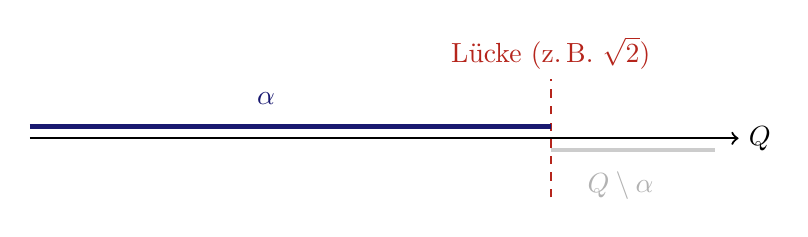
\begin{tikzpicture}[scale=1.5]
    % Q-Achse
    \draw[thick, ->] (-3,0) -- (3,0) node[right] {$\mathbb{Q}$};
    
    % Lücke bei Wurzel 2 (ca. 1.41)
    \coordinate (Gap) at (1.41, 0);
    \draw[dashed, BrickRed, thick] (Gap) ++(0,-0.5) -- ++(0,1) node[above] {Lücke (z.\,B. $\sqrt{2}$)};
    
    % Menge alpha (linker Teil)
    \draw[ultra thick, MidnightBlue] (-3,0.1) -- (1.41,0.1);
    \node[MidnightBlue, above] at (-1, 0.2) {$\alpha$};
    
    % Rechter Teil
    \draw[ultra thick, gray!40] (1.41,-0.1) -- (2.8,-0.1);
    \node[gray!60, below] at (2,-0.2) {$\mathbb{Q} \setminus \alpha$};
\end{tikzpicture}
\end{center}

\begin{explanation-of-steps}
Da die rationalen Zahlen \qt{Löcher} aufweisen (wie etwa bei $\sqrt{2}$), kann man eine reelle Zahl als die Trennung der rationalen Zahlen in zwei Klassen auffassen. Ein Dedekindscher Schnitt $\alpha$ repräsentiert dabei alle rationalen Zahlen, die links von der Trennstelle liegen.
\end{explanation-of-steps}
\end{math-stroke}

\subsection{Definition des Dedekindschen Schnitts}

\begin{spoken-clean}[00:25:30 - 00:27:30]
Okay, das heißt, unsere reellen Zahlen werden eigentlich eine Teilmenge der Potenzmenge von $\mathbb{Q}$ sein. Wir wollen, dass das Folgende erfüllt ist:

\textbf{(D0):} $\alpha$ soll nicht die leere Menge sein, und $\alpha$ soll nicht ganz $\mathbb{Q}$ sein.

Dann die zweite Bedingung, \textbf{(D1)}: Falls $p$ in $\alpha$ liegt und $q$ eine rationale Zahl ist, sodass $q < p$ ist, dann ist auch $q$ in $\alpha$. Das heißt, sobald eine Zahl $p$ in $\alpha$ ist, sind alle kleineren Zahlen auch in $\alpha$. Man sagt oft, die Menge ist nach unten abgeschlossen.

Und die letzte Bedingung, \textbf{(D2)}: Für jedes $p$ in $\alpha$ existiert ein $q$ in $\alpha$, sodass $p < q$ ist. In anderen Worten: Wir wollen, dass $\alpha$ kein maximales Element enthält. Okay?
\end{spoken-clean}

\begin{math-stroke}[Definition: Dedekindscher Schnitt]
\begin{definition}[Dedekindscher Schnitt]\label{def:dedekind-schnitt}
Eine Teilmenge $\alpha \subseteq \mathbb{Q}$ heißt \newterm{Dedekindscher Schnitt}, wenn sie die folgenden drei Bedingungen erfüllt:
\begin{enumerate}[label=\textbf{(D\arabic*)}, start=0]
    \item \textbf{Nicht-Trivialität:} $\alpha \neq \emptyset$ und $\alpha \neq \mathbb{Q}$.
    \item \textbf{Abgeschlossenheit nach unten:} $\forall p \in \alpha \; \forall q \in \mathbb{Q} \colon (q < p \implies q \in \alpha)$.
    \item \textbf{Kein maximales Element:} $\forall p \in \alpha \; \exists q \in \alpha \colon (p < q)$.
\end{enumerate}
\end{definition}

\begin{explanation-of-steps}[Bedeutung der Bedingungen]
\begin{enumerate}[label=\textbf{(D\arabic*)}, start=0]
    \item  stellt sicher, dass der Schnitt eine echte Aufteilung der rationalen Zahlen darstellt.
    \item  erzwingt, dass $\alpha$ ein \qt{Anfangsstück} der rationalen Zahlen ist.
    \item  sorgt für eine eindeutige Darstellung. Ohne diese Bedingung könnte man eine rationale Zahl $r$ sowohl durch $\{q \in \mathbb{Q} \mid q < r\}$ als auch durch $\{q \in \mathbb{Q} \mid q \le r\}$ repräsentieren. Durch den Ausschluss des Maximums wählen wir die \qt{offene} Variante.
\end{enumerate}
\end{explanation-of-steps}
\end{math-stroke}

\subsection{Die Menge der reellen Zahlen}

\begin{spoken-clean}[00:27:30 - 00:29:45]
Genau. Die Bemerkung ist, was ich vorher schon gesagt habe: Ein Dedekind-Schnitt $\alpha$ teilt $\mathbb{Q}$ in zwei disjunkte Mengen. Man hat $\alpha$ und man hat das Komplement von $\alpha$. Wegen \textbf{(D1)} wissen wir, dass alles in $\alpha$ kleiner ist als alles im Komplement. Und wegen \textbf{(D2)} wissen wir: Wenn die Trennstelle eine rationale Zahl ist, dann gehört diese Zahl zum Komplement und nicht zu $\alpha$.

Das heißt, wir haben jetzt eine eindeutige Weise, jede Stelle auf der Zahlengeraden zu identifizieren, egal ob dort eine rationale Zahl sitzt oder eine Lücke ist. Wir definieren also:
\[ \mathbb{R} := \{ \alpha \subseteq \mathbb{Q} \mid \alpha \text{ ist ein Dedekind-Schnitt} \}. \]
Das ist unsere Menge der reellen Zahlen. Wir werden nun sehen, wie wir auf dieser Menge die Operationen Addition und Multiplikation sowie die Ordnungsrelation definieren können, sodass alle Körper- und Ordnungsaxiome erfüllt sind.

Insbesondere werden wir zeigen, dass dieses Modell tatsächlich das Vollständigkeitsaxiom erfüllt. Das ist der ganze Grund, warum wir diesen Aufwand mit den Mengen von rationalen Zahlen überhaupt betreiben: Wir wollen die Lücken füllen. Wir haben die Lücken aufgefüllt, indem wir die Lücken selbst als Mengen von rationalen Zahlen definiert haben. Ein sehr eleganter Trick von Dedekind.

Gut, wir machen hier eine kurze Pause und schauen uns dann gleich an, wie man mit diesen Schnitten rechnet.
\end{spoken-clean}

\begin{math-stroke}[Die Menge der reellen Zahlen]
\begin{definition}[Reelle Zahlen]\label{def:reelle-zahlen}
Die Menge der \newterm{reellen Zahlen} $\mathbb{R}$ ist definiert als die Menge aller Dedekindschen Schnitte:
\[ \mathbb{R} := \{ \alpha \in \mathcal{P}(\mathbb{Q}) \mid \alpha \text{ erfüllt \textbf{(D0)}, \textbf{(D1)}, \textbf{(D2)}} \} \]
\end{definition}
\end{math-stroke}

\subsection{Einbettung der rationalen Zahlen}

\begin{spoken-clean}[00:30:50 - 00:33:24]
Wir definieren jetzt also $\mathbb{R}$ als die Menge aller Dedekind-Schnitte von $\mathbb{Q}$. Gut. Und jetzt hätten wir natürlich gerne, dass die rationalen Zahlen in $\mathbb{R}$ enthalten sind. Hat jemand eine Idee, wie man das bewerkstelligen könnte? Oder wie sieht man natürlicherweise $\mathbb{Q}$ als Teilmenge von $\mathbb{R}$? Wie kann man eine rationale Zahl als Dedekind-Schnitt interpretieren? Ja?
\end{spoken-clean}

\begin{student-interaction}[Student Answer]
Die Menge der Zahlen, die kleiner sind als die Zahl.
\end{student-interaction}

\begin{spoken-clean}[00:30:50 - 00:33:24]
Genau! Wir können die Menge aller Zahlen anschauen, die strikt kleiner als eine gegebene Zahl sind. Also für ein $p \in \mathbb{Q}$ definieren wir $\alpha_p$ als die Menge aller $q \in \mathbb{Q}$, sodass $q < p$ ist.
\end{spoken-clean}

\begin{math-stroke}[Einbettung der rationalen Zahlen]
Für jede rationale Zahl $p \in \mathbb{Q}$ definieren wir den zugehörigen Schnitt:
\begin{equation}
\label{eq:rational-cut}
\alpha_p := \{ q \in \mathbb{Q} \mid q < p \}
\end{equation}

\begin{claim}\label{clm:alpha-p-is-cut}
Für jedes $p \in \mathbb{Q}$ ist $\alpha_p$ ein Dedekindscher Schnitt.
\end{claim}

\begin{short-proof}
Wir verifizieren die Bedingungen aus Definition \ref{def:dedekind-schnitt}:
\begin{itemize}
    \item \textbf{(D0):} Da $p-1 < p$, ist $p-1 \in \alpha_p \implies \alpha_p \neq \emptyset$. Da $p < p$ falsch ist, ist $p \notin \alpha_p \implies \alpha_p \neq \mathbb{Q}$.
    \item \textbf{(D1):} Sei $q \in \alpha_p$ (d.\,h. $q < p$) und $r \in \mathbb{Q}$ mit $r < q$. Aus der Transitivität folgt $r < p$, also $r \in \alpha_p$.
    \item \textbf{(D2):} Sei $q \in \alpha_p$, also $q < p$. Da $\mathbb{Q}$ dicht liegt, existiert ein $r \in \mathbb{Q}$ mit $q < r < p$. Dann ist $r \in \alpha_p$ und $q < r$. Somit hat $\alpha_p$ kein maximales Element.
\end{itemize}
\end{short-proof}
\end{math-stroke}

\begin{spoken-clean}[00:33:24 - 00:35:23]
Müssen wir noch beweisen, dass das tatsächlich ein Dedekind-Schnitt ist. Machen wir das mal gründlich. Also, \textbf{(D0)} ist okay: Die Menge ist nicht leer, man kann immer kleinere Zahlen finden. Wir müssen \textbf{(D1)} zeigen, aber das ist auch klar: Wenn $q \in \alpha_p$ ist und $r \in \mathbb{Q}$, sodass $r < q$ ist, dann folgt, dass $r < q$ und $q < p$ ist. Das heißt, $r$ ist auch strikt kleiner als $p$ und somit folgt, dass $r$ auch in $\alpha_p$ ist. Da ist nicht viel dahinter.
\end{spoken-clean}

\subsection{Injektion von \texorpdfstring{$\mathbb{Q}$}{Q} nach \texorpdfstring{$\mathbb{R}$}{R}}

\begin{spoken-clean}[00:35:23 - 00:37:12]
Und dann noch das Letzte: Wir müssen zeigen, dass die Menge kein größtes Element hat. Aber das ist auch nicht schwierig. Wenn wir $q \in \alpha_p$ haben, dann nehmen wir einfach $r$ als die Mitte zwischen $p$ und $q$ --- also $(p + q) / 2$. Das ist auch eine rationale Zahl. Dann liegt $r$ zwischen $q$ und $p$, das heißt $q < r$ und $r \in \alpha_p$.

Okay, das heißt, wir erhalten eine Injektion von $\mathbb{Q}$ in die reellen Zahlen. Aber die Sache ist, dass nicht alle Dedekind-Schnitte von dieser Form sind --- die meisten, wie wir schlussendlich sehen werden, sind nicht von dieser Form.
\end{spoken-clean}

\begin{math-stroke}[Injektion von \texorpdfstring{$\mathbb{Q}$}{Q} nach \texorpdfstring{$\mathbb{R}$}{R}]
Die Abbildung $\iota \colon \mathbb{Q} \to \mathbb{R}, p \mapsto \alpha_p$ ist eine Injektion.
\[ \mathbb{Q} \hookrightarrow \mathbb{R} \]
\begin{explanation-of-steps}
Dies zeigt, dass wir die rationalen Zahlen als Teilmenge der reellen Zahlen auffassen können. Die \qt{echten} reellen Zahlen sind diejenigen Schnitte, die nicht durch eine rationale Zahl $p$ als $\alpha_p$ darstellbar sind.
\end{explanation-of-steps}
\end{math-stroke}

\subsection{Beispiel: Die irrationale Zahl \texorpdfstring{$\sqrt{2}$}{Wurzel 2}}

\begin{spoken-clean}[00:37:12 - 00:39:57]
Nehmen wir zum Beispiel Wurzel $2$ gewissermaßen. Wie könnte man Wurzel $2$ als Dedekind-Schnitt definieren? Hat jemand eine Idee? Ja?
\end{spoken-clean}

\begin{student-interaction}[Student Answer]
Die Menge aller rationalen Zahlen, deren Quadrat kleiner als 2 ist.
\end{student-interaction}

\begin{spoken-clean}[00:37:12 - 00:39:57]
Genau! Wir können zuerst sagen: Elemente in $\mathbb{R} \setminus \mathbb{Q}$ heißen irrational. Und das Beispiel ist: Wir können den Dedekind-Schnitt $\alpha$ anschauen, der aus allen $p \in \mathbb{Q}$ besteht, sodass $p^2 < 2$ ist. Und das definieren wir als $\sqrt{2}$.
\end{spoken-clean}

\begin{math-stroke}[Beispiel: Die irrationale Zahl \texorpdfstring{$\sqrt{2}$}{Wurzel 2}]
Elemente in $\mathbb{R} \setminus \iota(\mathbb{Q})$ heißen \newterm{irrationale Zahlen}.

\begin{example}[Der Schnitt für $\sqrt{2}$]\label{ex:sqrt-2-cut}
Wir definieren den Dedekindschen Schnitt für $\sqrt{2}$ durch:
\begin{equation}
\label{eq:sqrt-2-def}
\alpha_{\sqrt{2}} := \{ p \in \mathbb{Q} \mid p < 0 \lor p^2 < 2 \}
\end{equation}
\end{example}

\begin{explanation-of-steps}[Warum die Bedingung $p < 0$?]
Ein Dedekindscher Schnitt muss nach unten unbeschränkt sein (Bedingung \textbf{(D1)}). Würden wir nur $p^2 < 2$ fordern, lägen negative Zahlen wie $-3$ nicht in der Menge, obwohl sie kleiner als $\sqrt{2}$ sind. Daher nehmen wir alle negativen rationalen Zahlen explizit mit auf.
\end{explanation-of-steps}
\end{math-stroke}

\subsection{Irrationalität von \texorpdfstring{$\sqrt{2}$}{Wurzel 2}}

\begin{spoken-clean}[00:39:57 - 00:43:12]
Jetzt müssen wir natürlich noch beweisen, dass das tatsächlich ein Dedekind-Schnitt ist, und dann auch schauen, ob... ja, später müssten wir noch eine Multiplikation definieren und dann prüfen, dass wenn man diese Zahl mit sich selbst multipliziert, das tatsächlich $2$ ergibt. Das ist auf dem Übungsblatt diese Woche. Es ist nicht schwierig, aber es ist gut, so etwas einmal zu tun.

Um zu zeigen, dass das ein Dedekind-Schnitt ist, kann man sehen, dass es eben keine rationale Zahl gibt, die die Wurzel von $2$ ist. Wir wollen jetzt nochmals beweisen --- die Behauptung ist: Es gibt keine Zahl $p/q \in \mathbb{Q}$ (wobei $p$ und $q$ ganze Zahlen sind), sodass $p^2 / q^2 = 2$ ist.
\end{spoken-clean}

\begin{math-stroke}[Irrationalität von \texorpdfstring{$\sqrt{2}$}{Wurzel 2}]
\begin{proposition}\label{prop:sqrt-2-irrational}
Es existiert keine rationale Zahl $x \in \mathbb{Q}$ mit $x^2 = 2$.
\end{proposition}
\end{math-stroke}

\begin{spoken-clean}[00:43:12 - 00:45:42]
Beweis. Den Beweis, den man normalerweise sieht, verwendet die Primfaktorzerlegung. Hier haben wir einen Beweis, der von Dedekind stammt; deswegen ist das vielleicht passend für diesen Hörsaal und dieses Thema. Beweis von Dedekind.

Wir nehmen wieder an --- das ist wieder ein Widerspruchsbeweis ---: Nehmen wir an, es existieren solche $p, q \in \mathbb{N}$. Wir können annehmen, dass das natürliche Zahlen sind, weil diese hier auf jeden Fall beide positiv sind. Wir können also annehmen, dass $p, q \in \mathbb{N}$ liegen, sodass $p^2 / q^2 = 2$ ist. Das heißt mit anderen Worten: wir haben $p^2 - 2q^2 = 0$.

Wir nehmen jetzt an, dass $q \in \mathbb{N}$ die kleinste Zahl ist, die das erfüllt. Also die kleinste Zahl, sodass wenn wir $q^2$ nehmen und das mal $2$ rechnen, eine Quadratzahl herauskommt.
\end{spoken-clean}

\begin{proof}[Beweis von \cref{prop:sqrt-2-irrational} (nach Dedekind)]
\begin{spoken-clean}[00:45:42 - 00:48:12]
Was wir hier sehen: $p$ muss kleiner sein als $2q$. Wenn wir das Quadrat davon nehmen und das $2$ ergibt, muss es kleiner sein. Und wir wissen aber, dass $q < p$ ist. Auch hier wieder: das sind ganze Zahlen, das heißt, das Quadrat ist immer größer als die Zahl selbst.

Und jetzt definieren wir $\bar{q}$ als die Differenz $p - q$ und $\bar{p}$ als die Differenz $2q - p$. Das sind beides positive Zahlen. Wegen dem da haben wir hier, dass das wieder positiv ist: also $0 < \bar{q}$ und $\bar{q} < q$.

Was wir jetzt tun, ist zu zeigen, dass $2\bar{q}^2$ auch wieder ein Quadrat ist. Dazu rechnen wir einfach $\bar{p}^2 - 2\bar{q}^2$. Füllen wir das hier ein, die Definition: $\bar{p}^2$ ergibt $4q^2 - 4pq + p^2$. Und dann schauen wir uns $-2\bar{q}^2$ an, das ergibt $-2 \cdot (p^2 - 2pq + q^2)$. Sie schreien, wenn ich einen... ja?
\end{spoken-clean}

\begin{student-interaction}[Student Answer]
Nein, andersrum, oder? $q < p$. $q < p$, weil wenn wir $q^2$ nehmen und mit $2$ multiplizieren, bekommen wir $p^2$. Das passt.
\end{student-interaction}

\begin{math-stroke}[Widerspruchsbeweis: Unendlicher Abstieg]
Angenommen, es gäbe $p, q \in \mathbb{N}$ mit $\frac{p^2}{q^2} = 2$. Wir wählen $q$ minimal mit dieser Eigenschaft. Aus $1 < \sqrt{2} < 2$ folgt $q < p < 2q$.

Wir definieren neue Zahlen:
\begin{align}
\bar{q} &:= p - q \label{eq:q-bar} \\
\bar{p} &:= 2q - p \label{eq:p-bar}
\end{align}
Wegen $q < p < 2q$ gilt $0 < \bar{q} < q$. Wir berechnen nun:
\begin{align*}
\bar{p}^2 - 2\bar{q}^2 &= (2q - p)^2 - 2(p - q)^2 \\
&= (4q^2 - 4pq + p^2) - 2(p^2 - 2pq + q^2) \\
&= 4q^2 - 4pq + p^2 - 2p^2 + 4pq - 2q^2 \\
&= 2q^2 - p^2
\end{align*}
Da nach Annahme $p^2 = 2q^2$ gilt, folgt:
\[ \bar{p}^2 - 2\bar{q}^2 = 0 \implies \frac{\bar{p}^2}{\bar{q}^2} = 2 \]
Dies ist ein Widerspruch zur Minimalität von $q$, da $\bar{q} < q$.
\end{math-stroke}
\end{proof}

\begin{spoken-clean}[00:48:12 - 00:50:42]
Das kann man jetzt umschreiben, das ergibt $-p^2 + 2q^2$. Das hier fällt weg: $-2p^2$ und $p^2$ ergibt $-p^2$, und $4q^2 - 2q^2$ ergibt $2q^2$. Da wissen wir aber, dass das $0$ ist. Das heißt, $2\bar{q}^2$ ist tatsächlich eine Quadratzahl --- das kann aber nicht sein. \inlinemetanote{zeigt auf die Minimalität}

Das ist ein Widerspruch zur Minimalität von $q$. Okay, das beendet den Beweis. Immer gut, hin und wieder einen Rechenfehler zu machen, dann beginnen die Leute wieder mitzudenken. Sehr gut. Jetzt machen wir eine Pause und beginnen um Viertel nach wieder.
\end{spoken-clean}

\begin{lecture-break}[Pause]
Der Dozent kündigt eine Pause an. Die Vorlesung wird nach der Pause mit der Definition der Körperstruktur auf $\mathbb{R}$ fortgesetzt.
\end{lecture-break}

\section{Körperstruktur und Ordnung auf \texorpdfstring{$\mathbb{R}$}{R}}

\subsection{Addition von Dedekindschen Schnitten}

\begin{spoken-clean}[00:50:42 - 00:53:12]
Hier noch eine kleine Ergänzung zu dem, was wir vor der Pause kurz gemacht haben. Wir müssen hier nehmen... wir wissen $p < 2q$, das folgt direkt daraus, dass $p^2 = 2q^2$ ist. Und $q < p$. Damit folgt dann, dass $\bar{q}$, das wir als $p - q$ definiert haben, zwischen $0$ und $q$ liegt. Okay? Jetzt braucht es diese zwei Ungleichungen.

Als Nächstes wollen wir die Körperstruktur auf $\mathbb{R}$ definieren. Das Ziel ist nun: Definiere die Körperstruktur auf $\mathbb{R}$. Idealerweise wollen wir natürlich, dass das die Körperstruktur von $\mathbb{Q}$, das wir jetzt als Teilmenge von $\mathbb{R}$ aufgefasst haben, erweitert. Die Einschränkung auf $\mathbb{Q}$ soll also die übliche Körperstruktur ergeben.

Beginnen wir mit... okay, das ist ein bisschen eine längliche Sache. Wir machen zuerst die Addition. Das soll eine binäre Funktion auf $\mathbb{R}$ sein. Jetzt müssen wir sagen: Was ist $\alpha + \beta$? Hat jemand eine Idee, wie man das sinnvoll definieren könnte? Ja?
\end{spoken-clean}

\begin{student-interaction}[Student Answer]
Genau, das ist die Grundidee. Wir nehmen einfach alle $p + q$, wobei $p \in \alpha$ und $q \in \beta$ ist. Wir nehmen also einfach alle möglichen Kombinationen; das ist eine neue Menge, und das definieren wir als die Addition.
\end{student-interaction}

\begin{math-stroke}[Addition von Dedekindschen Schnitten]
\begin{definition}[Addition]\label{def:addition-cuts}
Für zwei Dedekindsche Schnitte $\alpha, \beta \in \mathbb{R}$ definieren wir ihre \newterm{Summe} durch:
\begin{equation}
\label{eq:addition-def}
\alpha + \beta := \{ p + q \mid p \in \alpha \land q \in \beta \}
\end{equation}
\end{definition}

\begin{lemma}\label{lem:addition-well-defined}
Falls $\alpha, \beta \in \mathbb{R}$, dann ist auch $\alpha + \beta \in \mathbb{R}$.
\end{lemma}
\end{math-stroke}

\begin{spoken-clean}[00:53:12 - 00:55:29]
Zuerst müssen wir prüfen, dass das wieder ein Dedekind-Schnitt ist. Ist das wieder ein Dedekind-Schnitt? Schnell überlegen. Machen wir das mal alle. Ich kann es kurz erklären, aber solche Sachen macht man in der Regel am besten alleine. Das Lemma ist jetzt: $\alpha + \beta$ ist ein Dedekind-Schnitt.

Der Beweis ist... okay, wir müssen einfach alle Axiome nachprüfen. \textbf{(D0)} ist eigentlich klar: Wir wissen, dass $\alpha$ und $\beta$ nicht die leere Menge sind. Das heißt, es gibt ein Element $p \in \alpha$ und $q \in \beta$. Daraus folgt, dass $p + q$ in $\alpha + \beta$ liegt, und somit ist das nicht leer. Das ist gut. Dann müssen wir noch zeigen, dass es nicht ganz $\mathbb{Q}$ ist.

Dazu nehmen wir einfach ein Element $r$, das in $\mathbb{Q}$ liegt, aber nicht in $\alpha$, und ein $s$, das in $\mathbb{Q}$ liegt, aber nicht in $\beta$. Dann gilt für alle $p \in \alpha$ und $q \in \beta$, dass $p < r$ und $q < s$ ist. Das muss für alle $p$ und $q$ gelten, weil sonst wäre ja $r$ in $\alpha$ enthalten oder $s$ in $\beta$. Somit folgt, dass $p + q < r + s$ ist. Das heißt, $r + s$ ist nicht in $\alpha + \beta$. Somit ist $\alpha + \beta$ nicht ganz $\mathbb{Q}$.
\end{spoken-clean}

\begin{proof}[Beweis von \cref{lem:addition-well-defined}]
\begin{math-stroke}[Nachweis von \textbf{(D0)}]
\textbf{(D0) Nicht-Trivialität:}
\begin{itemize}
    \item \textbf{Nicht leer:} Da $\alpha, \beta \neq \emptyset$, existieren $p \in \alpha$ und $q \in \beta$. Dann ist $p + q \in \alpha + \beta$, also $\alpha + \beta \neq \emptyset$.
    \item \textbf{Ungleich $\mathbb{Q}$:} Da $\alpha, \beta \neq \mathbb{Q}$, existieren $r \in \mathbb{Q} \setminus \alpha$ und $s \in \mathbb{Q} \setminus \beta$. Da Schnitte nach unten abgeschlossen sind, gilt für alle $p \in \alpha$ und $q \in \beta$: $p < r$ und $q < s$. Daraus folgt $p + q < r + s$. Somit ist $r + s \notin \alpha + \beta$, also $\alpha + \beta \neq \mathbb{Q}$.
\end{itemize}
\end{math-stroke}

\begin{math-stroke}[Nachweis von \textbf{(D1)}]
\textbf{(D1) Abgeschlossenheit nach unten:} Sei $x \in \alpha + \beta$ (d.\,h. $x = p + q$ mit $p \in \alpha, q \in \beta$) und $y \in \mathbb{Q}$ mit $y < x$. Wir setzen $p' := y - q$. Dann ist $p' + q = y$. Wegen $y < x = p + q$ folgt $p' + q < p + q \implies p' < p$. Da $\alpha$ ein Schnitt ist, folgt aus $p' < p$ und $p \in \alpha$, dass $p' \in \alpha$. Somit ist $y = p' + q \in \alpha + \beta$.
\end{math-stroke}

\begin{spoken-clean}[00:55:30 - 00:57:15]
Wir müssen noch zeigen --- wir hatten ja vor der Pause die Addition definiert ---, dass es kein maximales Element gibt. Wie können wir das machen? Können Sie schnell überlegen, während ich die Tafel putze? Hat jemand einen Vorschlag? Ja?
\end{spoken-clean}

\begin{student-interaction}[Student Answer]
Genau, genau! Es gab schon vorher keines, dann gibt es auch in der Summe keines. Wenn wir $r = p + q$ in $\alpha + \beta$ haben (mit $p \in \alpha, q \in \beta$), dann gibt es ein $p' \in \alpha$ mit $p < p'$, und daraus folgt, dass unser $r < p' + q$ ist, aber das ist immer noch in $\alpha + \beta$.
\end{student-interaction}

\begin{math-stroke}[Nachweis von \textbf{(D2)} für die Summe]
\textbf{(D2) Kein maximales Element:} Sei $r \in \alpha + \beta$ beliebig. Nach Definition der Summe existieren $p \in \alpha$ und $q \in \beta$ mit $r = p + q$.
\begin{itemize}
    \item Da $\alpha$ ein Dedekindscher Schnitt ist, erfüllt $\alpha$ die Bedingung \textbf{(D2)}. Somit existiert ein $p' \in \alpha$ mit $p < p'$.
    \item Wir betrachten nun $r' := p' + q$. 
\end{itemize}
Da $p' \in \alpha$ und $q \in \beta$, folgt nach Definition \eqref{eq:addition-def}, dass $r' \in \alpha + \beta$. Wegen $p < p'$ gilt zudem:
\[ r = p + q < p' + q = r'. \]
Somit haben wir zu jedem $r \in \alpha + \beta$ ein strikt größeres Element $r' \in \alpha + \beta$ gefunden. Die Menge $\alpha + \beta$ besitzt folglich kein maximales Element.
\end{math-stroke}
\end{proof}

\subsection{Das additive Inverse und die Subtraktion}

\begin{spoken-clean}[00:57:15 - 00:59:45]
Das Nullelement haben wir ja bereits. Was ist das Nullelement? Das haben wir gesagt: das sind alle $p \in \mathbb{Q}$, sodass $p < 0$ ist. Okay.

Jetzt ist die Frage: Wie können wir das Negative von $\alpha$ nehmen? Wenn wir $\alpha$ haben, was ist $-\alpha$? Für $\alpha \in \mathbb{R}$ definieren wir $-\alpha$ als den Dedekind-Schnitt, gegeben durch... wie könnte man das machen? Ja?
\end{spoken-clean}

\begin{student-interaction}[Student Answer]
Ja, man hätte gerne so ein bisschen wie alles auf dieser Seite, aber negativ genommen, damit es sich dann immer zu etwas kleinerem als Null addiert. Aber das ist ein bisschen schwierig, weil wir ja hier auch wieder etwas Größeres brauchen. Das ist genau die Idee mit dem Spiegeln eigentlich. Man kann es so hinschreiben: Wir nehmen alle $p \in \mathbb{Q}$, sodass für alle $q \in \alpha$ gilt $q + p < 0$.
\end{student-interaction}

\begin{spoken-clean}[01:02:20 - 01:04:45]
Das ist genau die Idee mit dem Spiegeln eigentlich. Man kann es auch anders hinschreiben. Man muss auch wieder schauen, dass das tatsächlich ein Dedekind-Schnitt ist. Kann man nachprüfen. Und somit können wir auch subtrahieren. Okay.

Gut, und dann können wir sagen, was es heißt, größer oder kleiner als Null zu sein. Wir sagen, $\alpha > 0$, falls... ein einfaches Kriterium, um zu sagen, dass $\alpha > 0$ ist? Ja?
\end{spoken-clean}

\begin{student-interaction}[Student Answer]
Genau, falls $0 \in \alpha$ ist. Wenn wir etwas nehmen, das kleiner als Null ist, und wir addieren Null dazu, dann ist es immer noch kleiner als Null. Das ist okay; ich glaube, es ist so etwas, womit wir die Null ausschließen.
\end{student-interaction}

\begin{spoken-clean}[01:04:45 - 01:07:15]
Wir sagen $\alpha > 0_{\mathbb{R}}$, falls $0 \in \alpha$ ist. Und $\alpha < 0_{\mathbb{R}}$, falls $-\alpha > 0_{\mathbb{R}}$ ist. Größer-gleich ist natürlich dann klar, was es bedeutet. Okay.

Und jetzt für die Multiplikation. Machen wir es vielleicht über die Multiplikation, da können wir sagen: wir multiplizieren mit $-1$, das geht vielleicht ganz gut. Was für Ideen gibt es für die Multiplikation? Ja?
\end{spoken-clean}

\begin{student-interaction}[Student Answer]
Genau, das ist die Grundidee. Das Problem ist halt mit den negativen Zahlen. Wenn beide positiv sind, dann ist das der richtige Weg. Da ist es ein bisschen eine mühsame Fallunterscheidung. Sagen wir, falls $\alpha, \beta \ge 0$ sind, so definieren wir $\alpha \cdot \beta$ als alle $p \cdot q$, sodass $p \in \alpha$ und $q \in \beta$ ist.
\end{student-interaction}

\begin{math-stroke}[Das additive Inverse]
\begin{definition}[Additives Inverses --- Naiver vs. korrekter Ansatz]\label{def:additives-inverses}
Der naive Ansatz zur Spiegelung eines Dedekindschen Schnitts $\alpha \in \mathbb{R}$,
\begin{equation}
\label{eq:additives-inverses-naive}
\textcolor{red}{-\alpha_{\text{naiv}} := \{ p \in \mathbb{Q} \mid \forall q \in \alpha \colon q + p < 0 \}} \quad \text{(\textcolor{red}{fehlerhaft für rationale Schnitte!})}
\end{equation}
erzeugt bei rationalen Schnitten ein maximales Element und verletzt damit Axiom \textbf{(D2)}.

Die präzise und korrekte Definition des \newterm{additiven Inversen} $-\alpha$ lautet:
\begin{equation}
\label{eq:additives-inverses-def}
-\alpha := \{ p \in \mathbb{Q} \mid \exists r \notin \alpha \colon p < -r \}
\end{equation}
\end{definition}

\begin{explanation-of-steps}
\textbf{Warum schlägt der naive Ansatz fehl?} Ist $\alpha = \alpha_s = \{q \in \mathbb{Q} \mid q < s\}$ ein rationaler Schnitt (z.\,B. $s = 1$), so würde $-s$ in $-\alpha_{\text{naiv}}$ liegen, da für alle $q < s$ gilt $q + (-s) < 0$. Damit wäre $-s$ ein größtes Element in $-\alpha_{\text{naiv}}$, was \textbf{(D2)} widerspricht. Die Bedingung $p < -r$ für ein $r \notin \alpha$ schließt das Maximum $-s$ strikt aus.
\end{explanation-of-steps}
\end{math-stroke}

\begin{ai-note}[Didaktische Analyse: Die Tücke beim Negativen eines Dedekind-Schnitts]
\textbf{Problem im naiven Ansatz:}
In der Vorlesung entsteht leicht die Idee, $-\alpha$ einfach durch $\{p \in \mathbb{Q} \mid \forall q \in \alpha \colon q + p < 0\}$ zu definieren.

\textbf{Mathematische Ursache des Fehlers:}
Betrachten wir den rationalen Schnitt $\alpha_s = \{q \in \mathbb{Q} \mid q < s\}$ für eine rationale Zahl $s \in \mathbb{Q}$:
\begin{itemize}
    \item Für $p = -s$ gilt für jedes $q \in \alpha$: $q + (-s) < s - s = 0$.
    \item Damit läge $-s$ in $-\alpha_{\text{naiv}}$, und $-s$ wäre das \emph{maximale Element} dieser Menge.
    \item Ein Dedekindscher Schnitt darf jedoch nach Axiom \textbf{(D2)} **kein maximales Element** besitzen!
\end{itemize}

\textbf{Die elegante Korrektur:}
Indem man Elemente $r \notin \alpha$ aus dem Komplement wählt und $p < -r$ fordert, wird die obere Grenze $-s$ strikt ausgeschlossen:
\[
-\alpha := \{ p \in \mathbb{Q} \mid \exists r \notin \alpha \colon p < -r \}
\]
Dies garantiert, dass $-\alpha$ nach unten abgeschlossen ist und kein größtes Element besitzt.
\end{ai-note}

\subsection{Die Ordnung auf den reellen Zahlen}
\begin{math-stroke}
\begin{definition}[Ordnung auf $\mathbb{R}$]\label{def:ordnung-reell}
Für zwei reelle Zahlen $\alpha, \beta \in \mathbb{R}$ definieren wir:
\begin{enumerate}[label=\textbf{(\roman*)}]
    \item \textbf{(i)} $\alpha \le \beta :\iff \alpha \subseteq \beta$
    \item \textbf{(ii)} $\alpha < \beta :\iff \alpha \subsetneq \beta$
\end{enumerate}
\end{definition}

\begin{remark}[Positivität]
\label{rem:positivitaet}
Eine reelle Zahl $\alpha$ ist genau dann positiv ($\alpha > 0_{\mathbb{R}}$), wenn $0 \in \alpha$. Wegen \textbf{(D2)} existiert dann ein rationales $q \in \alpha$ mit $q > 0$.
\end{remark}
\end{math-stroke}

\subsection{Multiplikation von Dedekindschen Schnitten}

\begin{spoken-clean}[01:07:15 - 01:10:00]
Wenn beide negativ sind, dann ist das ähnlich: dann nehmen wir einfach das Produkt von den Negativen, und dann geht es auch wieder auf. Also: falls $\alpha, \beta \le 0$ sind, definieren wir $\alpha \cdot \beta$ als $(-\alpha) \cdot (-\beta)$. Falls $\alpha \ge 0$ und $\beta \le 0$ ist, dann sagen wir $\alpha \cdot \beta$ ist $-(-\alpha \cdot -\beta)$, was immer das hier bedeutet. Und falls schließlich $\alpha \le 0$ und $\beta \ge 0$ ist, dann definieren wir $\alpha \cdot \beta$ als $-(-\alpha \cdot \beta)$.
\end{spoken-clean}

\begin{math-stroke}[Multiplikation von Dedekindschen Schnitten]
\begin{definition}[Multiplikation]\label{def:multiplikation-reell}
Seien $\alpha, \beta \in \mathbb{R}$.
\begin{itemize}
    \item \textbf{Fall 1 ($\alpha, \beta > 0_{\mathbb{R}}$):}
    \[ \alpha \cdot \beta := \{ p \in \mathbb{Q} \mid p < 0 \text{ oder } \exists q \in \alpha, r \in \beta \text{ mit } q, r > 0 \text{ und } p = q \cdot r \} \]
    \item \textbf{Fall 2 (Allgemeiner Fall):} Die Multiplikation wird unter Verwendung des additiven Inversen auf Fall 1 zurückgeführt:
    \[ \alpha \cdot \beta := \begin{cases} 
    0_{\mathbb{R}} & \text{falls } \alpha = 0_{\mathbb{R}} \lor \beta = 0_{\mathbb{R}} \\
    (-\alpha) \cdot (-\beta) & \text{falls } \alpha < 0_{\mathbb{R}} \land \beta < 0_{\mathbb{R}} \\
    -\bigl((-\alpha) \cdot \beta\bigr) & \text{falls } \alpha < 0_{\mathbb{R}} \land \beta > 0_{\mathbb{R}} \\
    -\bigl(\alpha \cdot (-\beta)\bigr) & \text{falls } \alpha > 0_{\mathbb{R}} \land \beta < 0_{\mathbb{R}}
    \end{cases} \]
\end{itemize}
\end{definition}

\begin{explanation-of-steps}
Im Skript wird die Multiplikation oft nur für positive reelle Zahlen explizit hingeschrieben, da die Fallunterscheidung für negative Zahlen rein technisch ist und keine neuen analytischen Einsichten liefert. Wichtig ist, dass bei der Multiplikation positiver Schnitte alle rationalen Zahlen $p < 0$ explizit mit aufgenommen werden, um die Bedingung \textbf{(D1)} (Abgeschlossenheit nach unten) zu erfüllen.
\end{explanation-of-steps}
\end{math-stroke}

\subsection{Die Körperstruktur von \texorpdfstring{$\mathbb{R}$}{R}}

\begin{spoken-clean}[01:10:00 - 01:12:45]
Das ist ein bisschen... ja, es lässt die Sache im Skript ein bisschen zu schön erscheinen, wenn man die negativen Zahlen weglässt. Aber es ist eben eine rein technische Angelegenheit. Was man jetzt eigentlich tun müsste, ist zu überprüfen, dass die Körperaxiome alle erfüllt sind. Man müsste also prüfen, dass das alles Dedekind-Schnitte sind und dass die Körperaxiome alle erfüllt sind. Sie können sich vorstellen, dass das eine sehr lange Angelegenheit ist.

Wir werden das jetzt nicht die nächsten drei Lektionen hier an der Tafel machen. Und ich erwarte auch nicht von Ihnen, dass Sie das machen. Aber falls Sie einmal eine lange Zugfahrt haben, können wir sagen: das ist eine gute Übung für eine lange Zugfahrt. Zeigen Sie, dass die reellen Zahlen --- also die Dedekind-Schnitte mit diesen Operationen --- die Körperaxiome erfüllen.
\end{spoken-clean}

\begin{math-stroke}[Die Körperstruktur von \texorpdfstring{$\mathbb{R}$}{R}]
\begin{theorem}\label{thm:reelle-zahlen-koerper}
Die Menge der reellen Zahlen $\mathbb{R}$ bildet mit der oben definierten Addition und Multiplikation einen angeordneten Körper, der die rationalen Zahlen $\mathbb{Q}$ (via der Einbettung $\iota \colon p \mapsto \alpha_p$) als Unterkörper enthält.
\end{theorem}

\begin{exercise}[Übung für lange Zugfahrten]
Verifizieren Sie die Körperaxiome $\mathbf{R_0}$ bis $\mathbf{R_{16}}$ für das Modell der Dedekindschen Schnitte. Zeigen Sie insbesondere die Gültigkeit des Distributivgesetzes:
\[ \alpha \cdot (\beta + \gamma) = \alpha \cdot \beta + \alpha \cdot \gamma \]
\end{exercise}
\end{math-stroke}

\subsection{Vollständigkeit von \texorpdfstring{$\mathbb{R}$}{R}}

\begin{spoken-clean}[01:12:45 - 01:15:30]
Was wir aber noch zeigen wollen, ist immerhin das $R_{17}$ --- wir wollen zumindest zeigen, dass es vollständig ist. Das ist ja der Grund, warum wir das Ganze machen. Die Behauptung ist: Die reellen Zahlen $\mathbb{R}$ erfüllen $R_{17}$. Das heißt, jede nichtleere, nach oben beschränkte Teilmenge $X$ hat ein Supremum.
\end{spoken-clean}

\begin{math-stroke}[Vollständigkeit von \texorpdfstring{$\mathbb{R}$}{R}]
\begin{theorem}[Vollständigkeitssatz]\label{thm:vollstaendigkeit-reell}
Das Modell der Dedekindschen Schnitte erfüllt das Vollständigkeitsaxiom $\mathbf{R_{17}}$.
\end{theorem}

\begin{short-proof}[Beweisidee]
Sei $X \subseteq \mathbb{R}$ eine nichtleere, nach oben beschränkte Menge von Dedekindschen Schnitten. Wir definieren den Kandidaten für das Supremum $\beta$ als die Vereinigung aller Schnitte in $X$:
\begin{equation}
\label{eq:supremum-konstruktion}
\beta := \bigcup X = \{ p \in \mathbb{Q} \mid \exists \alpha \in X \colon p \in \alpha \}
\end{equation}
\end{short-proof}
\end{math-stroke}

\begin{spoken-clean}[01:15:30 - 01:18:15]
Der Beweis ist dafür wirklich natürlich. Wir konstruieren das Supremum $\beta$ einfach als die Vereinigung von allen Dedekind-Schnitten in $X$. Zuerst müssen wir sehen, dass $\beta$ ein Dedekind-Schnitt ist. Dazu zeigen wir wieder alle drei Axiome.

\textbf{(D0):} Es ist klar, dass $\beta$ nicht leer ist, einfach da $X$ nicht leer ist und jedes $\alpha$ in $X$ nicht leer ist. Um zu zeigen, dass es nicht ganz $\mathbb{Q}$ ist, verwenden wir, dass $X$ nach oben beschränkt ist. Da $X$ nach oben beschränkt ist, gibt es ein $Q \in \mathbb{Q}$, sodass $p < Q$ für alle $p \in \beta$. Das heißt, $Q$ ist in $\mathbb{Q} \setminus \beta$. Somit ist $\beta$ nicht ganz $\mathbb{Q}$.

\textbf{(D1):} Das ist auch klar. Sei $p \in \beta$ und $q \in \mathbb{Q}$, sodass $q < p$ ist. Es existiert ein $\alpha \in X$, das $p$ enthält. Da $\alpha$ ein Dedekind-Schnitt ist, folgt daraus, dass $q$ auch in $\alpha$ enthalten ist. Und da $\alpha$ eine Teilmenge von $\beta$ ist, heißt das, dass $q$ auch in $\beta$ ist.

\textbf{(D2):} Wir müssen zeigen, dass es kein maximales Element gibt. Nehmen wir $p \in \beta$. Es existiert ein $\alpha \in X$, sodass $p \in \alpha$ ist. Da $\alpha$ ein Dedekind-Schnitt ist, folgt daraus, dass ein $q \in \alpha$ existiert, sodass $p < q$ ist. Und dann ist $q$ auch wieder in $\beta$ enthalten. Das heißt, unser $\beta$, das wir definiert haben, ist tatsächlich ein Dedekind-Schnitt.
\end{spoken-clean}

\begin{math-stroke}[Nachweis der Schnitteigenschaften für \texorpdfstring{$\beta$}{beta}]
\begin{enumerate}[label=\textbf{(D\arabic*)}, start=0]
    \item \textbf{Nicht-Trivialität:} 
    \begin{itemize}
        \item $\beta \neq \emptyset$, da $X \neq \emptyset$ (es existiert ein $\alpha \in X$) und $\alpha \neq \emptyset$.
        \item $\beta \neq \mathbb{Q}$, da $X$ nach oben beschränkt ist. Sei $\gamma \in \mathbb{R}$ eine obere Schranke, d.\,h. $\forall \alpha \in X \colon \alpha \subseteq \gamma$. Dann gilt $\beta = \bigcup_{\alpha \in X} \alpha \subseteq \gamma$. Da $\gamma \neq \mathbb{Q}$, folgt $\beta \neq \mathbb{Q}$.
    \end{itemize}
    \item \textbf{(Abgeschlossenheit nach unten:} Sei $p \in \beta$ und $q < p$. Dann $\exists \alpha \in X$ mit $p \in \alpha$. Da $\alpha$ ein Schnitt ist, folgt $q \in \alpha \subseteq \beta$.
    \item \textbf{Kein Maximum:} Sei $p \in \beta$. Dann $\exists \alpha \in X$ mit $p \in \alpha$. Da $\alpha$ kein Maximum hat, $\exists q \in \alpha$ mit $p < q$. Es folgt $q \in \beta$.
\end{enumerate}
\end{math-stroke}

\begin{spoken-clean}[01:18:15 - 01:21:00]
Jetzt müssen wir beweisen, dass es ein Supremum ist. Dazu müssen wir beweisen, dass es eine obere Schranke ist. Ist es klar, dass es eine obere Schranke ist? Da $\alpha \subseteq \beta$ für alle $\alpha \in X$ gilt, ist $\beta$ per Definition eine obere Schranke.

Was wir noch zeigen müssen, ist, dass es die kleinste obere Schranke ist. Dazu nehmen wir an, dass $\gamma \in \mathbb{R}$ beliebig ist, sodass $\gamma < \beta$ ist. Wenn $\gamma < \beta$ ist, dann ist $\gamma$ echt enthalten in $\beta$. Das heißt, wir können jetzt ein $p$ nehmen, das in $\beta$ liegt, aber nicht in $\gamma$. Dann wissen wir: es existiert ein $\alpha \in X$, das $p$ enthält. Daraus folgt jetzt aber, dass $\gamma < \alpha$, weil $\alpha$ ein Element enthält, das nicht in $\gamma$ enthalten ist. Das heißt, $\gamma$ ist keine obere Schranke für $X$.

Das beendet den Beweis. Die Vereinigung ist also genau das Supremum.
\end{spoken-clean}

\begin{math-stroke}[Nachweis der Supremums-Eigenschaft]
 \begin{enumerate}[label=\textbf{(\arabic*)}] 
    \item \textbf{$\beta$ ist eine obere Schranke:} Für jedes $\alpha \in X$ gilt $\alpha \subseteq \bigcup X = \beta$, also $\alpha \le \beta$.
    \item \textbf{$\beta$ ist die kleinste obere Schranke:} Sei $\gamma \in \mathbb{R}$ mit $\gamma < \beta$.
    \begin{itemize}
        \item $\gamma < \beta \implies \gamma \subsetneq \beta$.
        \item Es existiert also ein $p \in \beta \setminus \gamma$.
        \item Da $p \in \beta = \bigcup X$, existiert ein $\alpha \in X$ mit $p \in \alpha$.
        \item Da $p \in \alpha$ und $p \notin \gamma$, kann $\alpha \subseteq \gamma$ nicht gelten, d.\,h. $\alpha \not\le \gamma$.
    \end{itemize}
    Somit ist $\gamma$ keine obere Schranke für $X$. Folglich ist $\beta = \sup X$.
\end{enumerate}
\end{math-stroke}

\begin{didactic-insight}[Die Eleganz der Vereinigung]
Dieser Beweis offenbart die tiefe Eleganz der Dedekindschen Konstruktion: Das abstrakte analytische Konzept des Supremums (die \qt{kleinste obere Schranke}) kollabiert in der Mengentheorie auf die einfachste aller Operationen --- die Vereinigung ($\bigcup$). In $\mathbb{R}$ ist das Supremum einer Menge von Zahlen nichts anderes als die Menge aller rationalen Zahlen, die in mindestens einer dieser Zahlen enthalten sind.
\end{didactic-insight}

\subsection{Alternative Konstruktionen von \texorpdfstring{$\mathbb{R}$}{R}}

\begin{spoken-clean}[01:21:00 - 01:21:10]
Ich möchte zum Abschluss noch zwei Sachen erwähnen, und zwar gibt es noch andere Konstruktionen, die bekannt sind von den reellen Zahlen. Die bekannteste ist über Cauchy-Folgen. Das Problem ist ja mit den rationalen Zahlen, dass Cauchy-Folgen nicht unbedingt konvergieren. Und jetzt kann man sagen: Okay, wir wollen künstlich, dass alle Cauchy-Folgen konvergieren. Wie machen wir das? Wir nehmen einfach Äquivalenzklassen von Cauchy-Folgen und wir schauen uns all diese Äquivalenzklassen von Cauchy-Folgen an. Das ist die zweite klassische Konstruktion der reellen Zahlen. Die wurde fast gleichzeitig wie Dedekind auch publiziert; ich glaube, Cantor war das, der das gemacht hat.
\end{spoken-clean}

\begin{math-stroke}[Alternative Konstruktionen von \texorpdfstring{$\mathbb{R}$}{R}]
Es existieren weitere formale Wege, das Kontinuum der reellen Zahlen zu fundieren:
\begin{itemize}
    \item \textbf{Cauchy-Folgen (Cantor/Heine):} $\mathbb{R}$ wird als Menge der Äquivalenzklassen von rationalen Cauchy-Folgen definiert. Zwei Folgen sind äquivalent, wenn ihre Differenz eine Nullfolge ist.
    \item \textbf{Intervallschachtelungen:} Definition über Folgen von abgeschlossenen Intervallen, deren Länge gegen Null geht.
\end{itemize}
\end{math-stroke}

\subsection{Konstruktion aus \texorpdfstring{$\mathbb{Z}$}{Z} via quasi-linearer Funktionen}

\begin{spoken-clean}[01:21:10 - 01:21:17]
Und es gibt noch eine dritte, weniger bekannte, weniger klassische Konstruktion --- auch erst vor Kurzem entdeckt ---, und ich habe die auf das Übungsblatt diese Woche gesetzt. Das ist eine sehr nette Konstruktion, und zwar ist es eine Konstruktion der reellen Zahlen direkt aus den ganzen Zahlen. Man muss gar nicht zu den rationalen Zahlen gehen, sondern man kann die reellen Zahlen direkt aus den ganzen Zahlen konstruieren.

Die Idee ist, dass wir Äquivalenzklassen von quasi-linearen Funktionen anschauen. Das ist eine quasi-lineare Funktion, das heißt Funktionen $f$ von $\mathbb{Z}$ nach $\mathbb{Z}$, sodass die Menge von $f(n+m) - f(n) - f(m)$ (wobei $m, n$ ganze Zahlen sind) endlich ist. Wenn $f$ linear wäre, dann wäre das immer null. Wir schauen uns jetzt nur quasi-lineare an; das sind solche, bei denen diese Menge hier endlich ist. Da kann man jetzt Äquivalenzklassen von solchen geeigneten Äquivalenzklassen von quasi-linearen Funktionen anschauen, und da kann man zeigen, dass das auch wieder die reellen Zahlen ergibt. Das ist besonders elegant und natürlich, weil wir das direkt von den ganzen Zahlen aus machen können und gar nicht erst zu den rationalen Zahlen gehen müssen. Ich empfehle Ihnen, sich diese Übung ein bisschen anzuschauen, weil das noch interessant ist und nicht Standard.

Gut, vielen herzlichen Dank fürs Kommen und eine gute Woche!
\end{spoken-clean}

\begin{math-stroke}[Konstruktion aus \texorpdfstring{$\mathbb{Z}$}{Z} via quasi-linearer Funktionen]
\begin{definition}[Quasi-lineare Funktion]\label{def:quasi-linear}
Eine Funktion $f \colon \mathbb{Z} \to \mathbb{Z}$ heißt \newterm{quasi-linear}, wenn die Menge ihrer \qt{Defekte} endlich (beschränkt) ist:
\[ \{ f(n+m) - f(n) - f(m) \mid n, m \in \mathbb{Z} \} \text{ ist eine endliche Menge.} \]
\end{definition}

\begin{explanation-of-steps}
Man kann zeigen, dass der Quotient der Menge aller quasi-linearen Funktionen modulo der Äquivalenzrelation $f \sim g \iff \{f(n) - g(n) \mid n \in \mathbb{Z}\} \text{ ist endlich}$ isomorph zum Körper der reellen Zahlen $\mathbb{R}$ ist. Diese Konstruktion (oft \qt{Eudoxus-Reelle-Zahlen} genannt) fundiert das Kontinuum direkt auf der diskreten Struktur der ganzen Zahlen.
\end{explanation-of-steps}
\end{math-stroke}

\begin{nice-box}[Zusammenfassung der Schlüsselkonzepte]
In dieser Vorlesung haben wir die folgenden zentralen Punkte behandelt:
\begin{itemize}
    \item \textbf{Fundierungsaxiom:} Schließt unendliche $\in$-Abstiege und Zyklen aus, was die Mengenlehre strukturell bereinigt.
    \item \textbf{Axiomatik von $\mathbb{R}$:} Die reellen Zahlen sind charakterisiert als ein vollständig angeordneter Körper.
    \item \textbf{Dedekindsche Schnitte:} Eine reelle Zahl wird als ein nach unten abgeschlossenes Anfangsstück $\alpha \subsetneq \mathbb{Q}$ ohne maximales Element definiert.
    \item \textbf{Vollständigkeit:} Im Modell der Dedekindschen Schnitte entspricht das Supremum einer Menge einfach deren mengentheoretischer Vereinigung.
    \item \textbf{Einbettung:} Rationale Zahlen $p$ werden als Schnitte $\alpha_p = \{q \in \mathbb{Q} \mid q < p\}$ identifiziert.
\end{itemize}
\end{nice-box}